\documentclass{beamer}
\usetheme{Singapore}
\usepackage[utf8]{inputenc}
\usecolortheme{crane}
\usepackage{graphicx}
\usepackage{iwona}
\usepackage{standalone}
\usepackage{tikz}
\usetikzlibrary{arrows}
\usetikzlibrary{decorations.markings}
\usetikzlibrary{calc}
\usetikzlibrary{shapes,snakes}
\usepackage{amsmath}
\usepackage{amsfonts}
\usepackage{amsthm}
\usepackage{mathtools}
\usepackage{tcolorbox}
\usepackage{float}
\usepackage{bm}
\usepackage{minted}

\definecolor{lightblue}{RGB}{124,190,255}
\definecolor{darkgreen}{RGB}{24,145,0}
\definecolor{darkorange}{RGB}{220,110,0}



\beamertemplatenavigationsymbolsempty
\setbeamerfont{caption}{size=\tiny}


\title
{Simulating Queues with Ciw}
\author{Geraint Ian Palmer}
\date{PyCon Namibia 2016}
\titlegraphic{
\includegraphics[width=2.35cm]{cflogo} $\quad$ 
\includegraphics[width=2.35cm]{ciw_logo} $\quad$ 
\includegraphics[width=2.3cm]{napycon_logo} $\quad$ 
\includegraphics[width=2.3cm]{pydifflogo}}



\begin{document}

\frame{\titlepage}

\begin{frame}
\frametitle{What is a Queue?}
\begin{figure}
  \includestandalone[width=0.8\textwidth]{1nodeexample}
\end{figure}
\end{frame}

\begin{frame}
\begin{figure}
    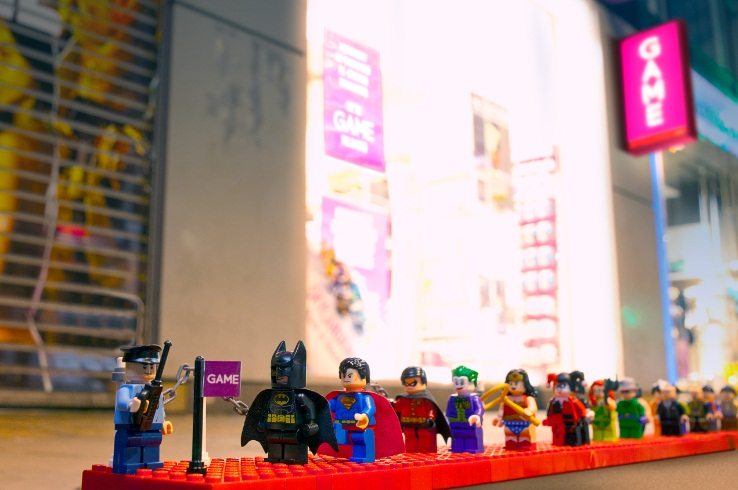
\includegraphics[width=\textwidth]{legoqueue}
\end{figure}
\end{frame}

\begin{frame}
\frametitle{What is a Queue?}
\begin{figure}
  \includestandalone[width=0.8\textwidth]{2nodefeedbackexample}
\end{figure}
\end{frame}


\begin{frame}
\begin{figure}
    \includestandalone[width=0.35\textwidth]{repostructure_code}
\end{figure}
\end{frame}

\begin{frame}
\frametitle{Three-Phase Simulation Approach}
\begin{figure}
    \includestandalone[width=\textwidth]{3phaseapprach}
\end{figure}
\end{frame}

\begin{frame}
\frametitle{Event Types}
\begin{center}
\begin{figure}
    \includestandalone[width=0.9\textwidth]{events}
\end{figure}
\end{center}
\end{frame}

\begin{frame}
\frametitle{Sampling from a Probability Distribution}
\end{frame}

\begin{frame}
\frametitle{Code Structure}
\begin{figure}
    \includestandalone[width=\textwidth]{codestructure}
\end{figure}
\end{frame}

\begin{frame}
\frametitle{Pair Programing / Collaborative Work}
\begin{figure}
    \includegraphics[width=0.9\textwidth]{collabwork}
\end{figure}
\end{frame}

\begin{frame}
\frametitle{Git \& GitHub}
\begin{figure}

\includegraphics[width=0.5\textwidth]{gitlogo}

\includegraphics[width=0.5\textwidth]{octocat}
\end{figure}
\end{frame}

\begin{frame}
\frametitle{GitHub Issues}
\begin{figure}
    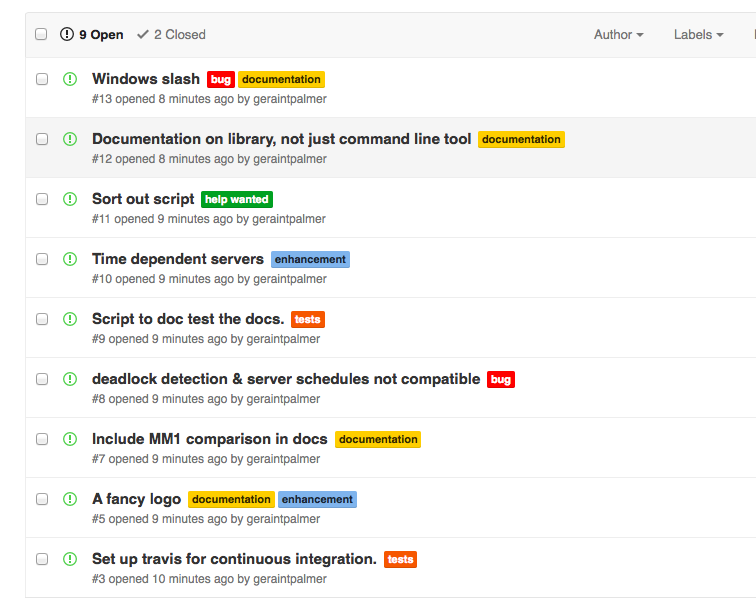
\includegraphics[width=0.8\textwidth]{githubissues}
\end{figure}
\end{frame}

\begin{frame}
\begin{figure}
    \includestandalone[width=0.35\textwidth]{repostructure_tests}
\end{figure}
\end{frame}

\begin{frame}
\frametitle{Doctests}
\inputminted{python}{doctests.py}
\end{frame}

\begin{frame}
\frametitle{Unittests}
\begin{center}
\fontsize{8.5pt}{10pt} \inputminted{python}{unittests.py}
\end{center}
\end{frame}

\begin{frame}
\frametitle{Travis}
\begin{columns}[c]
\column{.6\textwidth}
\begin{figure}[width=\colwidth]
    \vfill
    
\includegraphics[width=0.8\textwidth]{travispass}
    \vspace{10mm}
    
\includegraphics[width=0.8\textwidth]{travisfail}
    \vfill
\end{figure}
\column{.4\textwidth}
\begin{figure}[width=\textwidth]
    
\includegraphics[width=0.8\textwidth]{traviscilogo}
\end{figure}
\end{columns}
\end{frame}


\begin{frame}[fragile]
\frametitle{Coverage}
\fontsize{10pt}{10pt} \inputminted{python}{coverage.txt}
\end{frame}

\begin{frame}[fragile]
\frametitle{Coverage}
\fontsize{7pt}{9pt} \inputminted{python}{coverage_results.txt}
\end{frame}


\begin{frame}
\begin{figure}
    \includestandalone[width=0.35\textwidth]{repostructure_packaging}
\end{figure}
\end{frame}

\begin{frame}
\frametitle{Packaging}
\begin{center}
    \huge\texttt{pip install ciw}
\end{center}
\end{frame}

\begin{frame}
\begin{figure}
    \includestandalone[width=0.35\textwidth]{repostructure_docs}
\end{figure}
\end{frame}

\begin{frame}
\frametitle{Documentation}
\begin{figure}
    
\includegraphics[width=0.8\textwidth]{sphinxlogo}
\end{figure}
\begin{figure}
    
\includegraphics[width=0.8\textwidth]{readthedocslogo}
\end{figure}
\end{frame}


\begin{frame}
\frametitle{Academic Uses}
\vfill
\begin{block}{Theoretical Work}
Investigating deadlock in queueing networks.\\
(Geraint Palmer, Prof. Paul Harper, Dr. Vincent Knight)
\end{block}
\vfill
\begin{block}{Practical Work}
Modelling an ophthalmology clinic to strategise scheduling.\\
(Lieke H\"{o}lscher, Dr. Jennifer Morgan)
\end{block}
\vfill
\end{frame}


\begin{frame}
\frametitle{Investigating Deadlock}
\begin{figure}
    \includestandalone[width=\textwidth]{deadlock_digraph}
\end{figure}
\end{frame}

\begin{frame}
\begin{figure}
    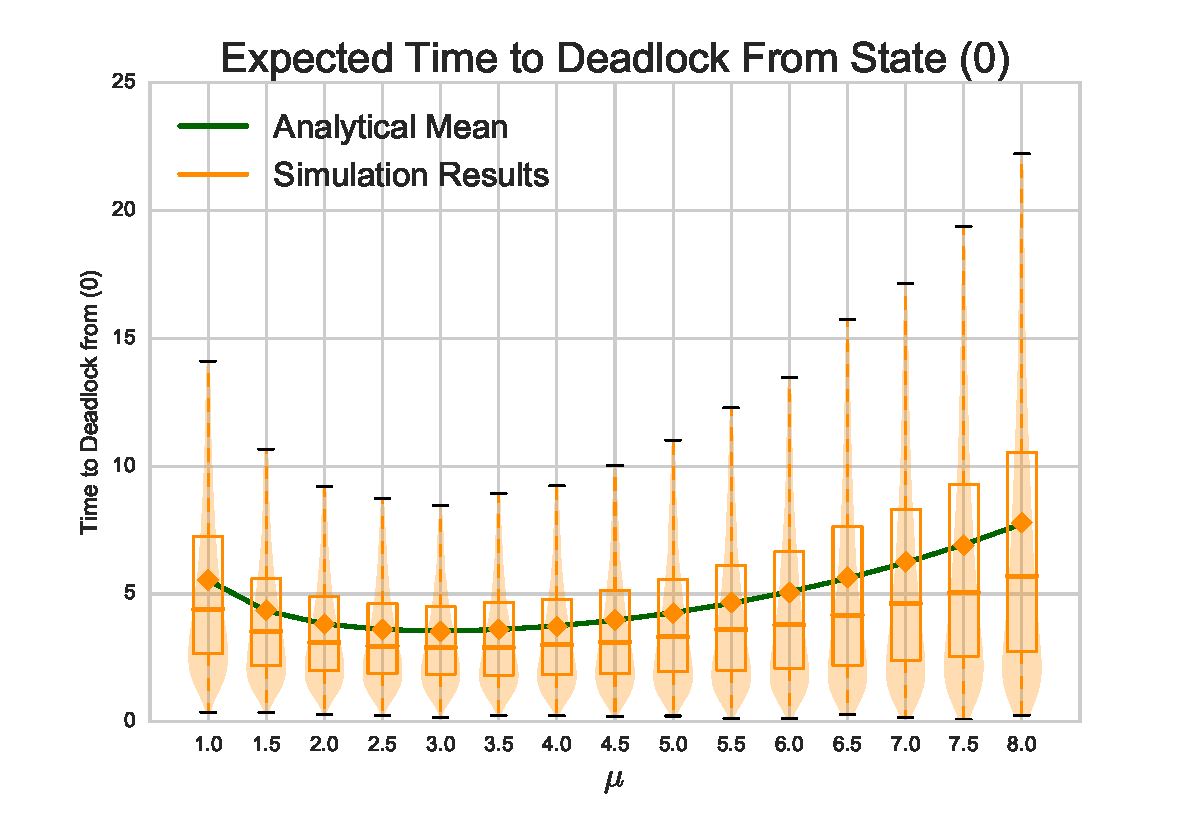
\includegraphics[width=\textwidth]{varymu_1Nms}
\end{figure}
\end{frame}

\begin{frame}
\frametitle{Modelling Ophthalmology Clinic}
\begin{figure}
    \includestandalone[width=0.9\textwidth]{ophthalmology}
\end{figure}
\end{frame}

\begin{frame}
\begin{columns}[b]
\begin{column}{.7\textwidth}
\begin{flushright}
\huge Thank You!\\[10mm]
\footnotesize palmergi1@cardiff.ac.uk\\[5mm]
\footnotesize \url{geraintianpalmer.org.uk}\\[5mm]
\footnotesize \url{github.com/geraintpalmer/Ciw}\\[5mm]
\footnotesize \url{ciw.readthedocs.org}\\[5mm]
\end{flushright}
\end{column}
\vrule{}
\begin{column}{.25\textwidth}
\begin{flushright}
\footnotesize PyYAML\\[1.75mm]
\footnotesize NetworkX\\[1.75mm]
\footnotesize Docopt\\[1.75mm]
\footnotesize Coverage\\[1.75mm]
\footnotesize TravisCI\\[1.75mm]
\footnotesize Sphinx\\[1.75mm]
\footnotesize ReadTheDocs\\[1.75mm]
\end{flushright}
\end{column}
\begin{column}{0.05\textwidth}
\end{column}
\end{columns}
\end{frame}

\end{document}
